\documentclass[11pt]{article}
\usepackage[a4paper,margin=1in]{geometry}
\usepackage{graphicx}
\usepackage{amsmath}
\usepackage{xcolor}
\usepackage{fancyhdr}
\usepackage{wrapfig}
\usepackage{titlesec}
\usepackage{array}
\definecolor{chapterblue}{RGB}{0,150,200}
\setlength{\headheight}{28pt}
\setlength{\headsep}{6pt}
\fancyhf{}
\fancyhead[L]{
\includegraphics[height=1.1cm]{../../iiitb_logo.png}}
\fancyhead[R]{%
\begin{tabular}{@{}r@{}}
\textbf{Name:} Pirjade Sabahat Rehan\\
\textbf{ID:} COMETFWC056\\
\textbf{Date:} February 1, 2026
\end{tabular}
}
\renewcommand{\headrulewidth}{0.8pt}
\renewcommand{\headrule}{%
\hbox to\headwidth{\color{chapterblue}\leaders\hrule height \headrulewidth\hfill}
}

\titleformat{\section}
{\color{chapterblue}\bfseries\large}
{\thesection}
{0.5em}
{}

\begin{document}
\thispagestyle{fancy}

\vspace*{-2pt}
\begin{center}
{\color{chapterblue}\Large\bfseries QUADRATIC EQUATIONS}
\end{center}

\noindent\textcolor{chapterblue}{\large\textbf{4.1 Introduction}}

In Chapter 2, you have studied different types of polynomials. One type was the
quadratic polynomial of the form $ax^2 + bx + c$, $a \neq 0$. When we equate this
polynomial to zero, we get a quadratic equation. Quadratic equations come up
when we deal with many real-life situations. For instance, suppose a charity
trust decides to build a prayer hall having a carpet area of $300$ square metres
with its length one metre more than twice its breadth. What should be the
length and breadth of the hall?

\begin{wrapfigure}{r}{0.40\textwidth}
\vspace{-10pt}
\centering
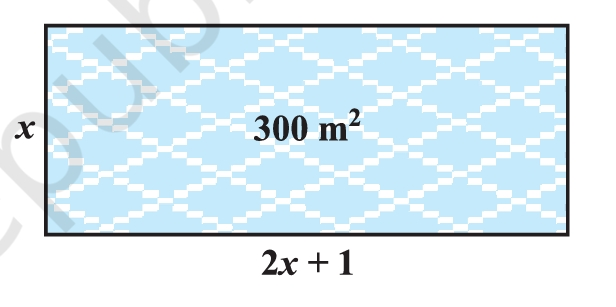
\includegraphics[width=0.38\textwidth]{figure/4.1.jpg}
\vspace{-6pt}
\textcolor{chapterblue}{Fig. 4.1}
\vspace{-10pt}
\end{wrapfigure}

Suppose the breadth of the hall is $x$ metres. Then, its length should be
$(2x + 1)$ metres. We can depict this information pictorially as shown in
Fig. 4.1.

\medskip

Now,\hfill area of the hall $= (2x + 1)\cdot x\ \text{m}^2 = (2x^2 + x)\ \text{m}^2$

\medskip

So,\hfill $2x^2 + x = 300$ \hfill (Given)

\medskip

Therefore,\hfill $2x^2 + x - 300 = 0$

\medskip

So, the breadth of the hall should satisfy the equation
$2x^2 + x - 300 = 0$ which is a quadratic equation.

\medskip

Many people believe that Babylonians were the first to solve quadratic
equations. For instance, they knew how to find two positive numbers with a
given positive sum and a given positive product, and this problem is equivalent
to solving a quadratic equation of the form $x^2 - px + q = 0$. Greek
mathematician Euclid developed a geometrical approach for finding out lengths
which, in our present day terminology, are solutions of quadratic equations.
Solving of quadratic equations, in general form, is often credited to ancient
Indian mathematicians. In fact, Brahmagupta (C.E.598–665) gave an explicit
formula to solve a quadratic equation of the form $ax^2 + bx = c$. Later,Sridharacharya (C.E. 1025) derived a formula, now known as the quadratic formula,
(as quoted by Bhaskara II) for solving a quadratic equation by the method of
completing the square. An Arab mathematician Al-Khwarizmi (about C.E. 800) also
studied quadratic equations of different types. Abraham bar Hiyya Ha-Nasi, in his
book `Liber embadorum' published in Europe in C.E. 1145 gave complete solutions of
different quadratic equations.

\medskip

In this chapter, you will study quadratic equations, and various ways of finding
their roots. You will also see some applications of quadratic equations in daily life
situations.

\noindent\textcolor{chapterblue}{\large\textbf{4.2 Quadratic Equations}}

A quadratic equation in the variable $x$ is an equation of the form
$ax^2 + bx + c = 0$, where $a$, $b$, $c$ are real numbers, $a \neq 0$.
For example,

\begin{center}
$2x^2 + x - 300 = 0$
\end{center}

is a quadratic equation. Similarly,

\begin{center}
$2x^2 - 3x + 1 = 0$, \quad $4x - 3x^2 + 2 = 0$ \quad and \quad $1 - x^2 + 300 = 0$
\end{center}

are also quadratic equations.

In fact, any equation of the form $p(x) = 0$, where $p(x)$ is a polynomial
of degree $2$, is a quadratic equation. But when we write the terms of $p(x)$
in descending order of their degrees, then we get the standard form of the
equation. That is,

\begin{center}
$ax^2 + bx + c = 0$, \quad $a \neq 0$
\end{center}

is called the \textbf{standard form of a quadratic equation}.

Quadratic equations arise in several situations in the world around us and in
different fields of mathematics. Let us consider a few examples.

\noindent\textcolor{chapterblue}{\textbf{Example 1:}} Represent the following situations mathematically:

\begin{enumerate}
\item John and Jivanti together have $45$ marbles. Both of them lost $5$ marbles
each, and the product of the number of marbles they now have is $124$. We would
like to find out how many marbles they had to start with.

\item A cottage industry produces a certain number of toys in a day. The cost of production of each toy (in rupees) was found to be $55$ minus the number of toys produced in a day. On a particular day, the total cost of production was $\textbf{Rs 750}$. We would like to find out the number of toys produced on that day.
\end{enumerate}

\noindent\textcolor{chapterblue}{\textbf{Solution:}}

\begin{enumerate}
\item Let the number of marbles John had be $x$. Then the number of marbles Jivanti had $= 45 - x$. The number of marbles left with John, when he lost $5$ marbles $= x - 5$. The number of marbles left with Jivanti, when she lost $5$ marbles
$= 45 - x - 5 = 40 - x$.
\end{enumerate}
Therefore, their product
\begin{center}
$= (x - 5)(40 - x)$
\end{center}
\begin{center}
$= 40x - x^2 - 200 + 5x$
\end{center}

\begin{center}
$= -x^2 + 45x - 200$
\end{center}
So,
\begin{center}
$-x^2 + 45x - 200 = 124$ \quad (Given that product = 124)
\end{center}

i.e.,

\begin{center}
$-x^2 + 45x - 324 = 0$
\end{center}
i.e.,
\begin{center}
$x^2 - 45x + 324 = 0$
\end{center}
Therefore, the number of marbles John had, satisfies the quadratic equation.
\begin{center}
$x^2 - 45x + 324 = 0$
\end{center}
which is the required representation of the problem mathematically.

\medskip
\noindent
(ii) Let the number of toys produced on that day be $x$.
Therefore, the cost of production (in rupees) of each toy that day $= 55 - x$.
So, the total cost of production (in rupees) that day

\begin{center}
$= x(55 - x)$
\end{center}

Therefore,

\begin{center}
$x(55 - x) = 750$
\end{center}

i.e.,

\begin{center}
$55x - x^2 = 750$
\end{center}

i.e.,

\begin{center}
$-x^2 + 55x - 750 = 0$
\end{center}

i.e.,

\begin{center}
$x^2 - 55x + 750 = 0$
\end{center}

Therefore, the number of toys produced that day satisfies the quadratic equation

\begin{center}
$x^2 - 55x + 750 = 0$
\end{center}

which is the required representation of the problem mathematically.
\medskip

\noindent\textcolor{chapterblue}{\textbf{Example 2:}} Check whether the following are quadratic equations:
\begin{enumerate}
\renewcommand{\labelenumi}{(\roman{enumi})}
\item $(x - 2)^2 + 1 = 2x - 3$ \item $x(x + 1) + 8 = (x + 2)(x - 2)$
\item $x(2x + 3) = x^2 + 1$ \item $(x + 2)^3 = x^3 - 4$
\end{enumerate}
\noindent
\textcolor{chapterblue}{\textbf{Solution:}}
\noindent
(i) LHS $= (x - 2)^2 + 1 = x^2 - 4x + 4 + 1 = x^2 - 4x + 5$
Therefore, $(x - 2)^2 + 1 = 2x - 3$ can be rewritten as
\begin{center}
$x^2 - 4x + 5 = 2x - 3$
\end{center}
i.e.,
\begin{center}
$x^2 - 6x + 8 = 0$
\end{center}

It is of the form $ax^2 + bx + c = 0$.
Therefore, the given equation is a quadratic equation.

\medskip
\noindent
(ii) Since $x(x + 1) + 8 = x^2 + x + 8$ and $(x + 2)(x - 2) = x^2 - 4$
Therefore,
\begin{center}
$x^2 + x + 8 = x^2 - 4$
\end{center}

i.e.,
\begin{center}
$x + 12 = 0$
\end{center}

It is not of the form $ax^2 + bx + c = 0$.
Therefore, the given equation is not a quadratic equation.

\medskip
\noindent
(iii) Here, \hspace{1cm} LHS $= x(2x + 3) = 2x^2 + 3x$
So,
\begin{center}
$x(2x + 3) = x^2 + 1$ can be rewritten as
\end{center}

\begin{center}
$2x^2 + 3x = x^2 + 1$
\end{center}
Therefore, we get
\begin{center}
$x^2 + 3x - 1 = 0$
\end{center}

It is of the form $ax^2 + bx + c = 0$.
So, the given equation is a quadratic equation.

\medskip
\noindent
(iv) Here, \hspace{1cm} LHS $= (x + 2)^3 = x^3 + 6x^2 + 12x + 8$

Therefore,
\begin{center}
$(x + 2)^3 = x^3 - 4$ can be rewritten as
\end{center}

\begin{center}
$x^3 + 6x^2 + 12x + 8 = x^3 - 4$
\end{center}

i.e.,
\begin{center}
$6x^2 + 12x + 12 = 0 \quad \text{or} \quad x^2 + 2x + 2 = 0$
\end{center}

It is of the form $ax^2 + bx + c = 0$.
So, the given equation is a quadratic equation.

\noindent\textcolor{chapterblue}{\textbf{Remark:}} Be careful! In (ii) above, the given equation appears to be a quadratic
equation, but it is not a quadratic equation. In (iv) above, the given equation appears to be a cubic equation (an equation of degree 3) and not a quadratic equation. But it turns out to be a quadratic equation. As you can see, often we need to simplify the given equation before deciding whether it is quadratic or not.

\begin{center}
\textcolor{chapterblue}{\Large\textbf{EXERCISE 4.1}}
\end{center}

\noindent
1. Check whether the following are quadratic equations:

\medskip
\noindent
\begin{tabular}{@{}p{0.47\textwidth} p{0.47\textwidth}@{}}
(i) $(x + 1)^2 = 2(x - 3)$
&
(ii) $x^2 - 2x = (-2)(3 - x)$
\\[6pt]

(iii) $(x - 2)(x + 1) = (x - 1)(x + 3)$
&
(iv) $(x - 3)(2x + 1) = x(x + 5)$
\\[6pt]

(v) $(2x - 1)(x - 3) = (x + 5)(x - 1)$
&
(vi) $x^2 + 3x + 1 = (x - 2)^2$
\\[6pt]

(vii) $(x + 2)^3 = 2x(x^2 - 1)$
&
(viii) $x^3 - 4x - x + 1 = (x - 2)^3$
\end{tabular}
\par
\medskip
\noindent
2. Represent the following situations in the form of quadratic equations:

\begin{enumerate}
\item[(i)] The area of a rectangular plot is $528\ \text{m}^2$. The length of the plot(in metres) is one more than twice its breadth. We need to find the length and
breadth of the plot.

\item[(ii)] The product of two consecutive positive integers is $306$. We need to
find the integers.

\item[(iii)] Rohan’s mother is $26$ years older than him. The product of their ages
(in years) $3$ years from now will be $360$. We would like to find Rohan’s present
age.

\item[(iv)] A train travels a distance of $480$ km at a uniform speed. If the speed
had been $8$ km/h less, then it would have taken $3$ hours more to cover the same distance. We need to find the speed of the train.
\end{enumerate}


\noindent\textcolor{chapterblue}{\large\textbf{4.3 Solution of a Quadratic Equation by Factorisation}}

Consider the quadratic equation $2x^2 - 3x + 1 = 0$.
If we replace $x$ by $1$ on the LHS of this equation, we get
$(2 \times 1^2) - (3 \times 1) + 1 = 0 = \text{RHS of the equation}$.
We say that $1$ is a root of the quadratic equation $2x^2 - 3x + 1 = 0$. This also means that $1$ is a zero of the quadratic polynomial
$2x^2 - 3x + 1$.

In general, a real number $\alpha$ is called a root of the quadratic equation
$ax^2 + bx + c = 0$, $a \neq 0$ if $a\alpha^2 + b\alpha + c = 0$.
We also say that $x = \alpha$ is a solution of the quadratic equation, or that
$\alpha$ satisfies the quadratic equation.
Note that the zeroes of the quadratic polynomial $ax^2 + bx + c$ and the roots
of the quadratic equation $ax^2 + bx + c = 0$ are the same.
You have observed, in Chapter~2, that a quadratic polynomial can have at most two zeroes. So, any quadratic equation can have at most two roots. You have learnt in Class~IX, how to factorise quadratic polynomials by splitting
their middle terms. We shall use this knowledge for finding the roots of a quadratic equation. Let us see how.

\medskip
\noindent\textcolor{chapterblue}{\textbf{Example 3:}}
Find the roots of the equation $2x^2 - 5x + 3 = 0$, by factorisation.

\medskip
\noindent\textcolor{chapterblue}{\textbf{Solution:}}
Let us first split the middle term $-5x$ as $-2x - 3x$
(because $(-2x) \times (-3x) = 6x^2 = (2x^2) \times 3$).
So,
$2x^2 - 5x + 3= 2x^2 - 2x - 3x + 3
= 2x(x - 1) - 3(x - 1)
= (2x - 3)(x - 1)$
Now, $2x^2 - 5x + 3 = 0$ can be rewritten as
$(2x - 3)(x - 1) = 0$
So, the values of $x$ for which $2x^2 - 5x + 3 = 0$ are the same for which
$(2x - 3)(x - 1) = 0$, i.e., either $2x - 3 = 0$ or $x - 1 = 0$.

Now, $2x - 3 = 0$ gives $x = \dfrac{3}{2}$ and $x - 1 = 0$ gives $x = 1$.
So, $x = \dfrac{3}{2}$ and $x = 1$ are the solutions of the equation.
In other words, $1$ and $\dfrac{3}{2}$ are the roots of the equation
$2x^2 - 5x + 3 = 0$.

\medskip
Verify that these are the roots of the given equation.
\noindent
\textbf{Note} that we have found the roots of $2x^2 - 5x + 3 = 0$ by factorising
$2x^2 - 5x + 3$ into two linear factors and equating each factor to zero.

\medskip
\noindent\textcolor{chapterblue}{\textbf{Example 4:}}
Find the roots of the quadratic equation $6x^2 - x - 2 = 0$.

\medskip
\noindent\textcolor{chapterblue}{\textbf{Solution:}}
We have

\begin{center}
$6x^2 - x - 2 = 6x^2 + 3x - 4x - 2$
\end{center}

\begin{center}
$= 3x(2x + 1) - 2(2x + 1)$
\end{center}

\begin{center}
$= (3x - 2)(2x + 1)$
\end{center}
The roots of $6x^2 - x - 2 = 0$ are the values of $x$ for which  
$(3x - 2)(2x + 1) = 0$.
Therefore, $3x - 2 = 0$ or $2x + 1 = 0$.

\medskip

i.e.,

\begin{center}
$x = \dfrac{2}{3} \quad \text{or} \quad x = -\dfrac{1}{2}$
\end{center}

Therefore, the roots of $6x^2 - x - 2 = 0$ are
$\dfrac{2}{3}$ and $-\dfrac{1}{2}$.

\medskip
We verify the roots, by checking that $\dfrac{2}{3}$ and $-\dfrac{1}{2}$
satisfy $6x^2 - x - 2 = 0$.

\medskip
\noindent\textcolor{chapterblue}{\textbf{Example 5:}}
Find the roots of the quadratic equation $3x^2 - 2\sqrt{6}x + 2 = 0$.

\medskip

\noindent\textcolor{chapterblue}{\textbf{Solution:}}

\begin{center}
$3x^2 - 2\sqrt{6}x + 2
= 3x^2 - \sqrt{6}x - \sqrt{6}x + 2$
\end{center}

\begin{center}
$= \sqrt{3}x(\sqrt{3}x - \sqrt{2}) -
\sqrt{2}(\sqrt{3}x - \sqrt{2})$
\end{center}

\begin{center}
$= (\sqrt{3}x - \sqrt{2})(\sqrt{3}x - \sqrt{2})$
\end{center}

So, the roots of the equation are the values of $x$ for which

\begin{center}
$(\sqrt{3}x - \sqrt{2})(\sqrt{3}x - \sqrt{2}) = 0$
\end{center}

Now, $\sqrt{3}x - \sqrt{2} = 0$ for

\begin{center}
$x = \sqrt{\dfrac{2}{3}}$
\end{center}

So, this root is repeated twice, one for each repeated factor
$\sqrt{3}x - \sqrt{2}$.

\medskip

Therefore, the roots of $3x^2 - 2\sqrt{6}x + 2 = 0$ are

\begin{center}
$\sqrt{\dfrac{2}{3}}, \; \sqrt{\dfrac{2}{3}}$
\end{center}

\noindent\textcolor{chapterblue}{\textbf{Example 6:}} Find the dimensions of the prayer hall discussed in Section 4.1.

\medskip

\noindent\textcolor{chapterblue}{\textbf{Solution:}}
In Section 4.1, we found that if the breadth of the hall is $x$ m, then $x$ satisfies the equation $2x^2 + x - 300 = 0$. Applying the factorisation method, we write this equation as

\begin{center}
$2x^2 - 24x + 25x - 300 = 0$
\end{center}

\begin{center}
$2x(x - 12) + 25(x - 12) = 0$
\end{center}

\begin{center}
$(x - 12)(2x + 25) = 0$
\end{center}

i.e.,

\begin{center}
$x = 12 \quad \text{or} \quad x = -12.5$
\end{center}

\noindent So, the roots of the given equation are $x = 12$ or $x = -12.5$. Since $x$ is the
breadth of the hall, it cannot be negative.

\noindent Thus, the breadth of the hall is $12$ m. Its length $= 2x + 1 = 25$ m.
\begin{center}
\textcolor{chapterblue}{\Large\textbf{EXERCISE 4.2}}
\end{center}
\medskip

\noindent
1. Find the roots of the following quadratic equations by factorisation:

\begin{tabular}{@{}p{0.48\textwidth} p{0.48\textwidth}@{}}
(i) $x^2 - 3x - 10 = 0$ 
& 
(ii) $2x^2 + x - 6 = 0$ \\[6pt]

(iii) $\sqrt{2}x^2 + 7x + 5\sqrt{2} = 0$ 
& 
(iv) $2x^2 - x - \dfrac{1}{8} = 0$ \\[6pt]

(v) $100x^2 - 20x + 1 = 0$ 
&
\end{tabular}

\medskip

\noindent
2. Solve the problems given in Example 1.

\medskip

\noindent
3. Find two numbers whose sum is $27$ and product is $182$.

\medskip

\noindent
4. Find two consecutive positive integers, sum of whose squares is $365$.

\medskip

\noindent
5. The altitude of a right triangle is $7$ cm less than its base.
If the hypotenuse is $13$ cm, find the other two sides.

\medskip

\noindent
6. A cottage industry produces a certain number of pottery articles in a day.It was observed on a particular day that the cost of production of each article(in rupees) was $3$ more than twice the number of articles produced on that day.If the total cost of production on that day was \text{Rs.}\,90, find the number of articles produced and the cost of each article.

\medskip
\noindent\textcolor{chapterblue}{\large\textbf{4.4 Nature of Roots}}

\medskip

\noindent The equation $ax^2 + bx + c = 0$ are given by

\begin{center}
$x = \dfrac{-b \pm \sqrt{b^2 - 4ac}}{2a}$
\end{center}

If $b^2 - 4ac > 0$, we get two distinct real roots
$\dfrac{-b}{2a} + \dfrac{\sqrt{b^2 - 4ac}}{2a}$ and
$\dfrac{-b}{2a} - \dfrac{\sqrt{b^2 - 4ac}}{2a}$.

If $b^2 - 4ac = 0$, then

\begin{center}
$x = \dfrac{-b \pm 0}{2a}$, i.e., $x = \dfrac{-b}{2a}$ or $\dfrac{-b}{2a}$.
\end{center}
So, the roots of the equation $ax^2 + bx + c = 0$ are both $\dfrac{-b}{2a}$. Therefore, we say that the quadratic equation $ax^2 + bx + c = 0$ has two equal real roots in this case. If $b^2 - 4ac < 0$, then there is no real number whose square is $b^2 - 4ac$.
Therefore, there are no real roots for the given quadratic equation in this case. Since $b^2 - 4ac$ determines whether the quadratic equation $ax^2 + bx + c = 0$ has real roots or not, $b^2 - 4ac$ is called the \textbf{discriminant} of the quadratic equation. So, a quadratic equation $ax^2 + bx + c = 0$ has

\begin{enumerate}
\item[(i)] \textbf{two distinct real roots}, if $b^2 - 4ac > 0$,
\item[(ii)] \textbf{two equal real roots}, if $b^2 - 4ac = 0$,
\item[(iii)] \textbf{no real roots}, if $b^2 - 4ac < 0$.
\end{enumerate}
Let us consider some examples.
\medskip

\noindent\textcolor{chapterblue}{\textbf{Example 7:}} Find the discriminant of the quadratic
equation $2x^2 - 4x + 3 = 0$, and hence find the nature of its roots.

\noindent\textcolor{chapterblue}{\textbf{Solution:}} The given equation is of the form
$ax^2 + bx + c = 0$, where $a = 2$, $b = -4$ and $c = 3$.
Therefore, the discriminant
\begin{center}
$b^2 - 4ac = (-4)^2 - 4(2 \times 3) = 16 - 24 = -8 < 0$.
\end{center}
So, the given equation has no real roots.
\medskip

\noindent\textcolor{chapterblue}{\textbf{Example 8:}} A pole has to be erected at a point on the
boundary of a circular park of diameter $13$ metres in such a way that the difference of its distances from two diametrically opposite fixed gates $A$ and $B$ on the boundary is $7$ metres. Is it possible to do so? If yes, at what distances from the two gates should the pole be erected?

\noindent\textcolor{chapterblue}{\textbf{Solution :}} Let us first draw the diagram (see Fig. 4.2).

\begin{wrapfigure}{r}{0.38\textwidth}
\centering
\vspace{-10pt}
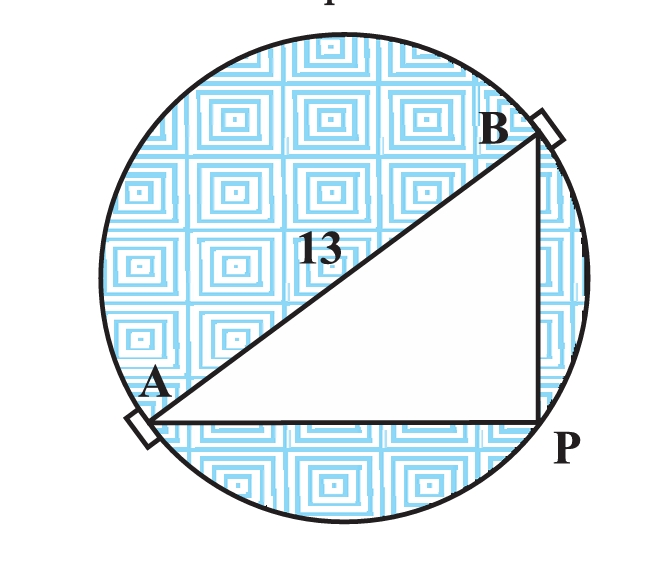
\includegraphics[width=0.38\textwidth]{figure/4.2.jpg}
\vspace{-10pt}
\end{wrapfigure}
Let $P$ be the required location of the pole.  
Let the distance of the pole from the gate $B$ be $x$ m, i.e., $BP = x$ m.

Now the difference of the distances of the pole from the two gates  
$= AP - BP$ (or, $BP - AP$) $= 7$ m.

Therefore,
$AP = (x + 7)\text{ m}$ 
Now, $AB = 13$ m, and since $AB$ is a diameter,

$\angle APB = 90^\circ$ (Why?)

Therefore,

$AP^2 + PB^2 = AB^2$ (By Pythagoras theorem)

i.e.,

\begin{center}
$(x + 7)^2 + x^2 = 13^2$
\end{center}

i.e.,

\begin{center}
$x^2 + 14x + 49 + x^2 = 169$
\end{center}

i.e.,

\begin{center}
$2x^2 + 14x - 120 = 0$
\end{center}

So, the distance $x$ of the pole from gate B satisfies the equation

\begin{center}
$x^2 + 7x - 60 = 0$.
\end{center}

So, it would be possible to place the pole if this equation has real roots.
To see if this is so or not, let us consider its discriminant.
The discriminant is

\begin{center}
$b^2 - 4ac = 7^2 - 4 \times 1 \times (-60) = 289 > 0$.
\end{center}

So, the given quadratic equation has two real roots, and it is possible to erect
the pole on the boundary of the park.

Solving the quadratic equation $x^2 + 7x - 60 = 0$, by the quadratic formula, we get

\begin{center}
$x = \dfrac{-7 \pm \sqrt{289}}{2} = \dfrac{-7 \pm 17}{2}$.
\end{center}
Therefore,

\begin{center}
$x = 5 \text{ or } -12$.
\end{center}

Since $x$ is the distance between the pole and the gate B, it must be positive.
Therefore, $x = -12$ will have to be ignored. So, $x = 5$. Thus, the pole has to be erected on the boundary of the park at a distance of
$5$ m from the gate B and $12$ m from the gate A.

\medskip
\noindent\textcolor{chapterblue}{\textbf{Example 9 :}}
Find the discriminant of the equation
$3x^2 - 2x + \dfrac{1}{3} = 0$ and hence find the nature of its roots.
Find them, if they are real.

\medskip
\noindent\textcolor{chapterblue}{\textbf{Solution :}}
Here $a = 3$, $b = -2$ and $c = \dfrac{1}{3}$.

\medskip
Therefore, discriminant

\begin{center}
$b^2 - 4ac = (-2)^2 - 4 \times 3 \times \dfrac{1}{3} = 4 - 4 = 0$.
\end{center}

Hence, the given quadratic equation has two equal real roots.

\medskip
The roots are $\dfrac{-b}{2a}, \dfrac{-b}{2a}$, i.e.,
$\dfrac{2}{6}, \dfrac{2}{6}$, i.e.,
$\dfrac{1}{3}, \dfrac{1}{3}$.
\begin{center}
\textcolor{chapterblue}{\Large\textbf{EXERCISE 4.3}}
\end{center}

\noindent
1. Find the nature of the roots of the following quadratic equations. If the real roots exist, find them:
\medskip
\begin{tabular}{@{}p{0.45\textwidth} p{0.45\textwidth}@{}}
(i) $2x^2 - 3x + 5 = 0$ 
& (ii) $3x^2 - 4\sqrt{3}\,x + 4 = 0$ \\[6pt]

(iii) $2x^2 - 6x + 3 = 0$ 
& ~
\end{tabular}

\medskip
\noindent
2. Find the values of $k$ for each of the following quadratic equations, so that they have two equal roots.

\medskip
\begin{tabular}{@{}p{0.45\textwidth} p{0.45\textwidth}@{}}
(i) $2x^2 + kx + 3 = 0$
& (ii) $kx(x - 2) + 6 = 0$
\end{tabular}

\medskip
\noindent
3. Is it possible to design a rectangular mango grove whose length is twice its breadth, and the area is $800\ \text{m}^2$? If so, find its length and breadth.

\medskip
\noindent
4. Is the following situation possible? If so, determine their present ages.  
The sum of the ages of two friends is 20 years. Four years ago, the product of their ages (in years) was 48.

\medskip
\noindent
5. Is it possible to design a rectangular park of perimeter 80 m and area $400\ \text{m}^2$? If so, find its length and breadth.

\medskip
\noindent
\textcolor{chapterblue}{\large\textbf{4.5 Summary}}

\medskip
\noindent In this chapter, you have studied the following points:

\medskip
\noindent
1. A quadratic equation in the variable $x$ is of the form
$ax^2 + bx + c = 0$, where $a$, $b$, $c$ are real numbers and $a \neq 0$.

\medskip
\noindent
2. A real number $\alpha$ is said to be a root of the quadratic equation
$ax^2 + bx + c = 0$, if $a\alpha^2 + b\alpha + c = 0$.
The zeroes of the quadratic polynomial $ax^2 + bx + c$ and the roots of the
quadratic equation $ax^2 + bx + c = 0$ are the same.

\medskip
\noindent
3. If we can factorise $ax^2 + bx + c$, $a \neq 0$, into a product of two linear
factors, then the roots of the quadratic equation $ax^2 + bx + c = 0$ can be
found by equating each factor to zero.

\medskip
\noindent
4. Quadratic formula: The roots of a quadratic equation
$ax^2 + bx + c = 0$ are given by
$
x = \frac{-b \pm \sqrt{b^2 - 4ac}}{2a},
$
provided $b^2 - 4ac \geq 0$.

\medskip
\noindent
5. A quadratic equation $ax^2 + bx + c = 0$ has

\medskip
\noindent
\hspace*{1em}(i) two distinct real roots, if $b^2 - 4ac > 0$,

\medskip
\noindent
\hspace*{1em}(ii) two equal roots (i.e., coincident roots), if $b^2 - 4ac = 0$, and

\medskip
\noindent
\hspace*{1em}(iii) no real roots, if $b^2 - 4ac < 0$.
\end{document}
